% !TEX TS-program = pdflatex
% !TEX encoding = UTF-8 Unicode

% This is a simple template for a LaTeX document using the "article" class.
% See "book", "report", "letter" for other types of document.

\documentclass[11pt]{paper} % use larger type; default would be 10pt

%%% Examples of Article customizations
% These packages are optional, depending whether you want the features they provide.
% See the LaTeX Companion or other references for full information.

%%% PAGE DIMENSIONS
%\usepackage{geometry} % to change the page dimensions
%\geometry{a4paper} % or letterpaper (US) or a5paper or....
% \geometry{margin=2in} % for example, change the margins to 2 inches all round
% \geometry{landscape} % set up the page for landscape
%   read geometry.pdf for detailed page layout information
\usepackage{mathtools}
\usepackage{graphicx} % support the \includegraphics command and options
\usepackage{caption}
\usepackage{subcaption}
\usepackage{wrapfig}

\usepackage[style=numeric-comp, sorting=none, url=false, isbn=false]{biblatex}
\addbibresource{binding-pocket.bib}

% \usepackage[parfill]{parskip} % Activate to begin paragraphs with an empty line rather than an indent

%%% PACKAGES
%\usepackage{booktabs} % for much better looking tables
%\usepackage{array} % for better arrays (eg matrices) in maths
%\usepackage{paralist} % very flexible & customisable lists (eg. enumerate/itemize, etc.)
%\usepackage{verbatim} % adds environment for commenting out blocks of text & for better verbatim
%\usepackage{subfig} % make it possible to include more than one captioned figure/table in a single float
% These packages are all incorporated in the memoir class to one degree or another...

%%% HEADERS & FOOTERS
%\usepackage{fancyhdr} % This should be set AFTER setting up the page geometry
%\pagestyle{fancy} % options: empty , plain , fancy
%\renewcommand{\headrulewidth}{0pt} % customise the layout...
%\lhead{}\chead{}\rhead{}
%\lfoot{}\cfoot{\thepage}\rfoot{}

%%% SECTION TITLE APPEARANCE
%\usepackage{sectsty}
%\allsectionsfont{\sffamily\mdseries\upshape} % (See the fntguide.pdf for font help)
% (This matches ConTeXt defaults)

%%% ToC (table of contents) APPEARANCE
%\usepackage[nottoc,notlof,notlot]{tocbibind} % Put the bibliography in the ToC
%\usepackage[titles,subfigure]{tocloft} % Alter the style of the Table of Contents
%\renewcommand{\cftsecfont}{\rmfamily\mdseries\upshape}
%\renewcommand{\cftsecpagefont}{\rmfamily\mdseries\upshape} % No bold!

%%% END Article customizations

%%% The "real" document content comes below...

\title{No title yet}
\author{Majid Saberi \and Hamed Seyed-allaei\thanks{hamed@ipm.ir}}
\institution{School of Cognitive Science, \\ Institute for Research in Fundamental Sciences (IPM), \\Tehran, Iran}
%\date{} % Activate to display a given date or no date (if empty),
         % otherwise the current date is printed 

\newcommand{\numberofreceptors}{32 }


\begin{document}
\maketitle

\begin{abstract}
	%The goal of this work is twofold: 
	%first we show that how olfactory receptor neurons respond to the molecular volume,
	%and after that, we infer some structural properties of the binding-pocket of olfactory receptors.
	The results of this study is essential to the study of olfactory coding and is helpful in calculations and/or measurements of 3D  structure of olfactory receptors proteins.
	In this work we show that the response of an olfactory receptor neurons in Drosophila depends on molecular volume of an odorant;  
	The molecular volume determines the upper limits of the neural response, 
	while the actual response depends on other properties of the molecules; 
	Therefore, it is important to correct the effect of molecular volume before studying molecular bases of olfactory responses.
	We show that this dependence can be described by a Gaussian function: 
	Each olfactory receptor prefers a particular volume (the mean), 
	with some degree of flexibility (the standard deviation). 
	These two parameters predict the volume and flexibility of the binding-pocket of the olfactory receptors, 
	which are the targets of structural biology studies; 
	Therefore, our results provide structural biologist with some additional information about the structure olfactory receptors. 
\end{abstract}

\section{Introduction}
\begin{figure}
	\centering
	\begin{subfigure}[b]{0.45 \textwidth}
		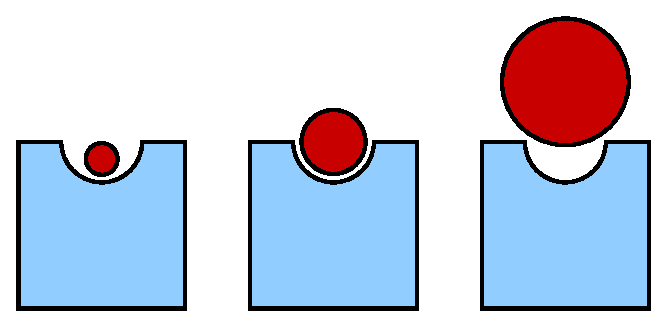
\includegraphics[width=\textwidth]{fig/binding-pocket}
		\caption{Binding-pocket volume}
		\label{fig:pocket-size}
	\end{subfigure}
	\begin{subfigure}[b]{0.45 \textwidth}
		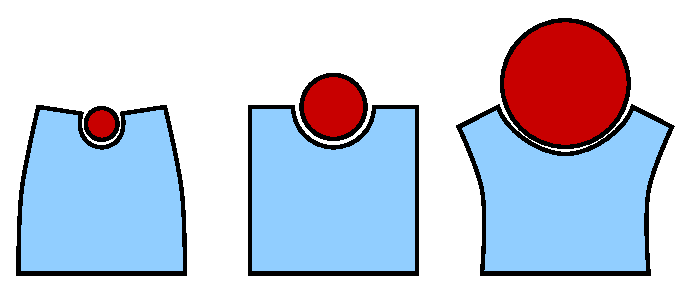
\includegraphics[width=\textwidth]{fig/binding-pocket-flex}
		\caption{Binding-pocket flexibility}
		\label{fig:pocket-flex}
	\end{subfigure}
	\caption{This figure shows different scenarios that may happen when an odorant molecule (ligand) binds to a receptor. 
		Fig. \ref{fig:pocket-size} shows the effect of binding-pocket volume. 
		From left to right, misfit because of small volume of molecule, perfect match and misfit because of large molecular volume.
		Fig. \ref{fig:pocket-flex} demonstrates that the flexibility of a receptor may compensate for the volume mismatches. 
		The red disks (dark grey in b\&w) are odorant molecule, 
		and the blue shapes (light grey in b\&w) are olfactory receptor and binding-pocket.}
	\label{fig:binding-pocket}
\end{figure}

Survival of many species depends on their olfactory system~\cite{}. 
They use it  to search for food~\cite{}, 
avoid poison~\cite{}, 
escape from danger~\cite{}, 
find mate~\cite{}, 
and bind to their offspring~\cite{}.
An olfactory system detects volatile chemicals in the surrounding, 
encodes the results and transmit them to limbic system and cortex~\cite{}.

The front end of the olfactory system are olfactory receptor neurons. 
Each neuron expresses only one kind of olfactory receptor, 
neurons of the same type converge into the same glomeruli of the olfactory bulb,
so that each glomerulus of olfactory bulb receives an amplified signal from only one type of olfactory receptor~\cite{}.
That makes the olfactory bulb (or antennal lobe in insects) the best place to record the effect of odorant molecules on the olfactory receptors. 
From these recording we know that the olfactory systems use a combinatorial code: 
an olfactory receptor can be triggered by different odorant molecules, 
and an odorant molecule can excite different olfactory receptors~\cite{Malnic2000}.  
However, it is not clear yet which properties of a molecule contribute to its smell,
it is a topic of ongoing researches and there are many theories~\cite{Turin,Vosshall2000,Araneda2000,Brookes2007,Franco2011,Pelz2006,Gabler2013}.

In this study, 
we investigate the relation between molecular volumes of odorants and the responses of olfactory receptor neurons. 
Our results suggest that molecular volume is a considerable factor, 
but not the only factor that determines the neural response of the olfactory receptor neurons.

The olfactory receptors are transmembrane proteins.
In vertebrates, thery are metabotropic receptors, they belong to the family of g-protein coupled receptor (GPCR), 
Linda B. Buck and Richard Axel won the Nobel Prize in Physiology or Medicine, in 2004, 
for the discovery of this~\cite{Buck1991}.
There are many similarities between the olfactory system of insects and vertebrates~\cite{Kaupp2010}, 
and it was assumed that insects use the same kind of signal transduction~\cite{}, 
but recently, XX and XX argued that the olfactory receptors in insects are inotropic~\cite{Sato2008,Wicher2008}. 

Regardless of the signal transduction, 
all olfactory receptor have the same function, they have a binding-pocket (also known as binding-cavity and binding-site),
where the ligands (odorants) bind to. 
This binding activates the receptors and
the activated receptor changes the potential of the cell, directly (inotropic) or indirectly (metabotropic).

The amount of change in the membrane potential of a olfactory receptor neuron depends on the number of activated olfactory receptor proteins and the time that they remain activated,
which are determined by various physio-chemical properties of the ligand (odorant) and the receptor~\cite{Khafizov2007,Lupieri2009}, 
but here we focus only on two of them: the volume and the flexibility of the binding-pocket.
The molecular volume of a ligand should match the dimensions of the binding-pocket of the receptor,
then it fits into the binding-pocket of the receptor and triggers the signal transduction. 
Any mismatch in the volumes will affect the neural responses (Fig. \ref{fig:pocket-size}), 
on the other hand the flexibility of the binding-pocket can compensate for the volume mismatch (Fig. \ref{fig:pocket-flex}),

We could know the volume and flexibility of the binding-pocket, if we knew its three dimensional structure.
But this is not the case here, it is not easy to know the structure of integral proteins~\cite{}, 
including olfactory receptor. It is the topic of ongoing researches, 
using various methods like Molecular Dynamic (MD) simulations~\cite{Khafizov2007,Lupieri2009}, 
mutagenesis studies~\cite{}, heterologus expression studies~\cite{}, and homology modeling~\cite{}.
In this study, we use neural recording to predict the volume and flexibility of binding-pocket of olfactory receptors, {\it in-vivo}.

In this study we suggest a functional relation between molecular volume and the neural responses, 
we provide a methodology to estimate {\it chemical range} or {\it tuning function} of olfactory receptors,
and then we predict the structural properties of the binding-pocket of olfactory receptor - the volume and the flexibility of binding-pocket.
Our results may help to odorant selection  of new experimental studies, 
may provide additional information about the structure of olfactory receptors to structural biologists, 
and may contribute to the study of olfactory coding.

To perform this study we use a public domain, well structured database -- DoOR -- 
that includes the neural responses of most olfactory receptors (OR) of Drosophila to many odorants~\cite{Galizia2010}. 
This database has collected its data from many other sources~\cite{Bruyne1999,Bruyne2001,Dobritsa2003,Goldman2005,Hallem2004,Hallem2006,
Kreher2005,Kreher2008,Kwon2007,Pelz2006,Pelz2006,Schmuker2007,Stensmyr2003,
Turner2009,VanderGoesvanNaters2007,Yao2005}.

%%

%There are many studies that tries to connect physio-chemical properties of molecules to their perceived smells, like the current work, which studies the effect of molecular volume of odorants on the response of olfactory receptors.

%The olfactory system of insects are similar to the olfactory system of vertebrates in many ways ...  They are also differences .... 

%Some receptors respond to few molecules, some response to many.

%Insects receptors neurons show spontaneos activity of 8 Hz.

%Drosophila's olfactory receptors are ionotropic. They may be metabotropic. It is under debate.

% They have seven trans-membrane domains. They need Or83b to work. 
% they may construct a complex that work as a cation channel or Or83b functions as cation channel and collaborte with Olfactory receptor.

% Olfactory receptor are presents in other organs like kindny ans sperms.

%chemical receptory range.

%in GPCR odorant interact with helix 2,7
%2-58 candidate residues.

%Drosophila about 60 receptors, mamals 300-1300 receptors. 

%In low concentraiotn the response is narrow. In high concentration the response is broad.

%OR67d Pheremone. 
%Odor prediciton from the shape.
%Olfactory white.



\section{Material and methods}
\begin{figure}
	\centering
	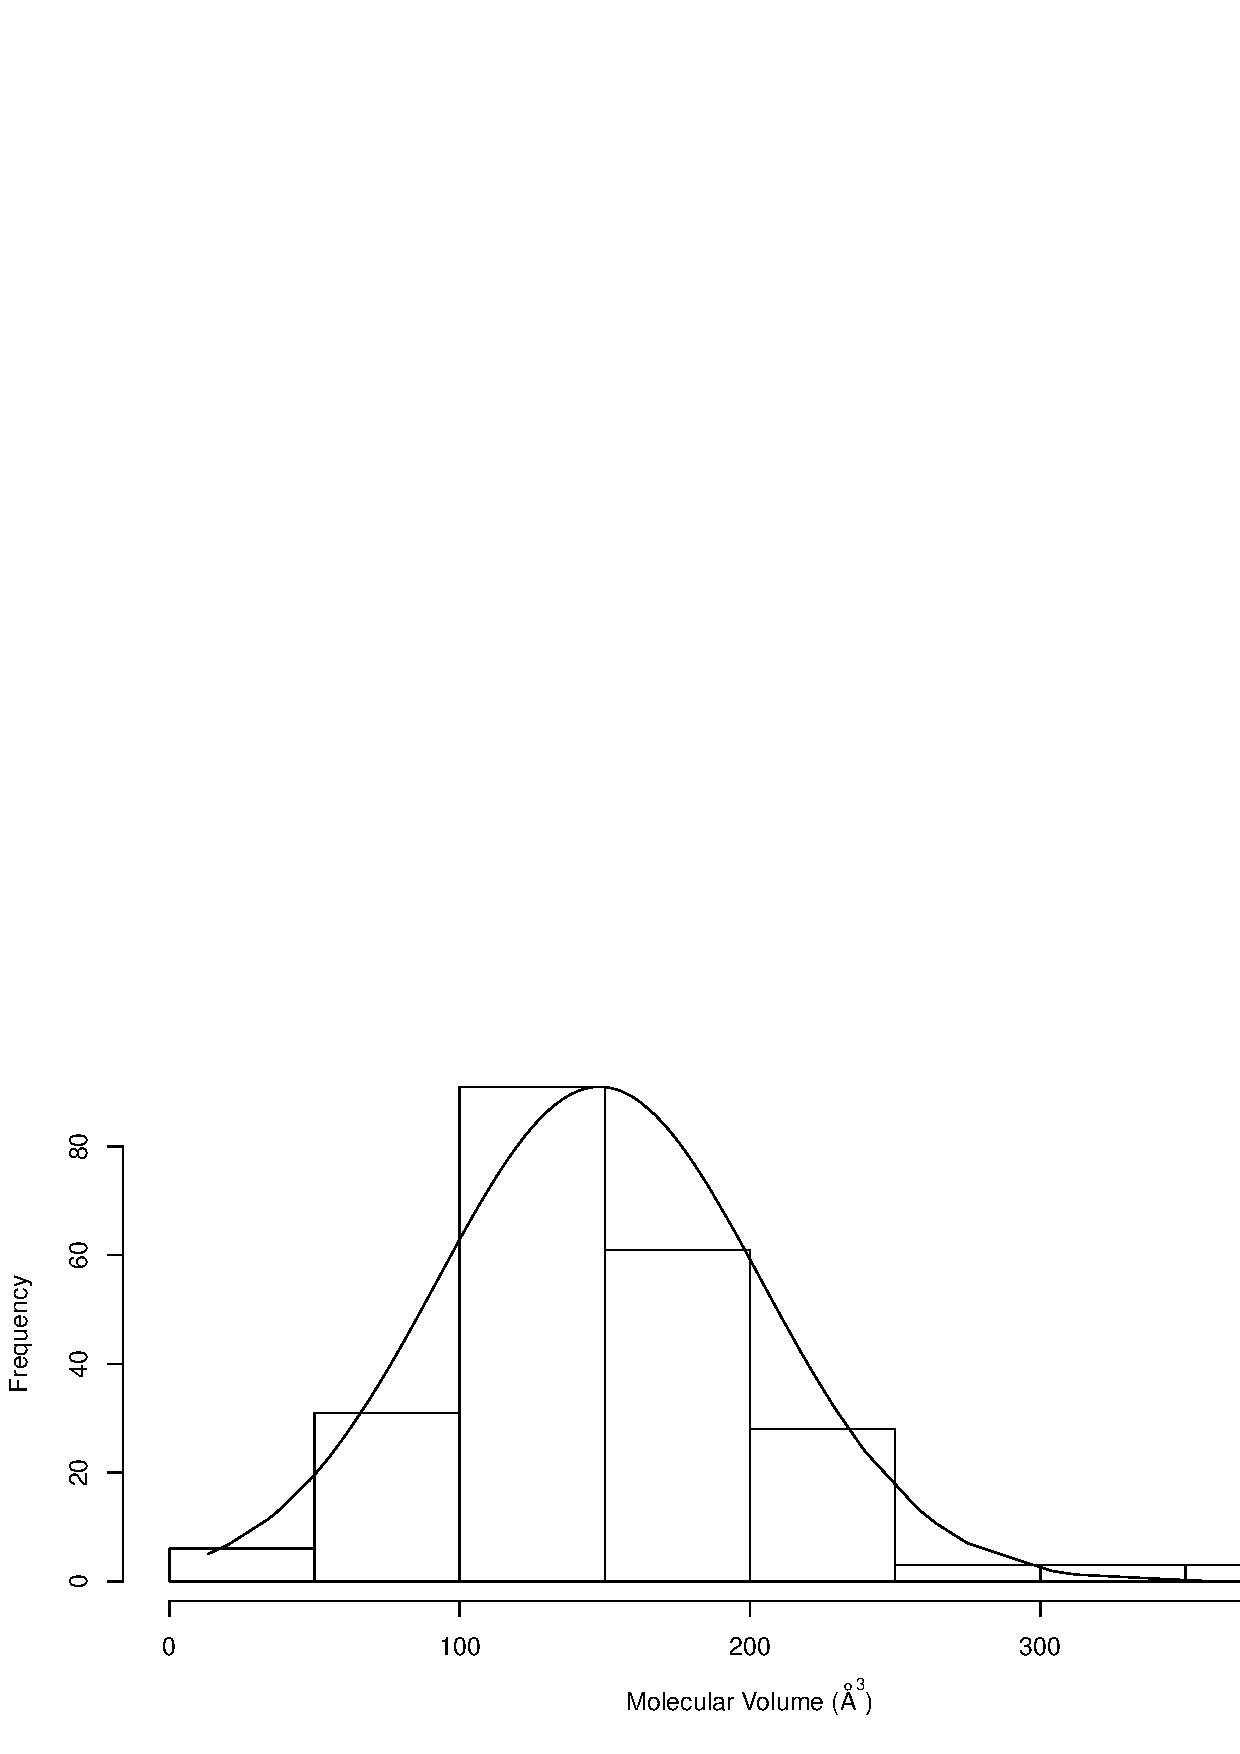
\includegraphics[width=0.5 \textwidth]{fig/hist-volumes}
	\caption{Density function of molecular volumes ($g(v)$), considering all molecules of DoOR database. 
		The actual density function of molecular of volumes in each experiment ($g(v)$) might be slightly different 
		because each experiment uses a different subset of molecules. 
		The solid line is a Gaussian fit (Eq. \ref{eqn:hist-volumes}).}
	\label{fig:hist-volumes}
\end{figure}

We want to study the relation between neural responses and molecular volumes, so we need the respective data. 
We take the neural data of DoOR database \cite{Galizia2010} and we calculate molecular volume using a computational chemistry software -- VEGA ZZ~\cite{}. 

DoOR database can be summarized in an $N\times M$ matrix. 
Its elements $r_{nm}$, are the response of neuron $n$ to odorant $m$. 
This matrix is normalized between 0 and 1 so we have $0 \le r_{nm} \le 1$, where 1 is the strongest response.
The only problem is that this matrix has some Not Available (NA) values, 
different neurons are excited by different set of odorants, 
so  when summing over $m$, $\sum_m$, we are calculating $\sum_{m: r_{nm} \neq \text{NA}}$, but for simplicity, 
we use the former notation. 

The response $r_{nm}$ depends on the molecular volume of the odorant, $v_m$, 
and other physio-chemical properties of the molecule $m$; 
We assume that we can separate the response $r_{nm}$ into two terms:
\begin{equation}
	r_{nm} = f_n(v_m) \psi_{nm}.
	\label{eqn:factors}
\end{equation}
The first term, $f_n(v_m)$, depends only on the molecular volume of odorants.
The second term, $\psi_{nm}$ include every other influential properties of molecules, but the molecular volume.
Both terms are characteristic of each receptor, and they might vary from neuron to neuron.
In fact, the first term, $f_n(v)$, is the tuning curve of neuron $n$ in respect to the molecular volumes, 
it can be approximated with a Gaussian function
\begin{equation}
	\displaystyle f_n(v) = e^{-\frac{(v-v_n)^2}{2\sigma^2_n}}, 
	\label{eqn:volume-dependence}
\end{equation}
where, $v_n$ is the preferred molecular volume of receptor $n$ and $\sigma_n$ represents its flexibility. 
In this work we want to estimate $v_n$ and $\sigma_n$. 
To do so, first we calculate the response weighted average of molecular volumes, 
$\frac{\sum_{m} v_m r_{nm}}{\sum_{m} r_{nm}}$ and then we use (\ref{eqn:factors}):
\begin{equation}
	\frac{\displaystyle \sum_{m} v_m r_{nm}}{\displaystyle \sum_{m} r_{nm}} = \frac{\displaystyle \sum_{m} v_m f_n(v_m) \psi_{nm}}{\displaystyle \sum_{m} f_n(v_m) \psi_{nm}}.
	\label{eqn:sta}
\end{equation}
Here we can approximate $\sum$ with $\int$, which is common in statistical physics~\cite{}:
\begin{equation}
	\sum_{m} \dots f_n(v_m) \psi_{nm} \approx  \langle \psi_{nm} \rangle_m \int_0^\infty \dots f_n(v) g(v)  dv. 
	\label{eqn:sigma_to_int}
\end{equation}
In which, 
$\langle \psi_{nm} \rangle_m$ denotes the average of $\psi_{nm}$ over all $m: r_{nm} \neq \text{NA}$. 
It can be moved out of the integral for it is independent of $v$.
In the above equation, 
$g(v)$ is the density of states, $g(v) dv$ indicates how many molecules have a molecular volume in the range of $v$ and $v+dv$.
This function can be approximated by a Gaussian function, Fig.\ref{fig:hist-volumes}, 
\begin{equation}
	g(v) = e^{-\frac{(v- v_{g})^2}{2 \sigma_{g}^2}},
	\label{eqn:hist-volumes}
\end{equation}
ideally, $g(v)$ should not depend on the neuron $n$, 
it is the property of ensemble of odorant molecules, not neurons. 
But here, we have many missing values ($r_{nm} = NA$), 
so we have to calculate $g(v)$ for each neuron separately; 
Therefore, $v_{g_n}$ and $\sigma_{g_n}$ are the average and standard deviation of molecular volume while $r_{nm} \neq \text{NA}$.
Now we rewrite equation (\ref{eqn:sta}) using equation (\ref{eqn:sigma_to_int}):
\begin{equation}
	\frac{\displaystyle \sum_{m} v_m r_{nm}}{\displaystyle \sum_{m} r_{nm}} \approx \frac{\displaystyle \int v f_n(v) g_n(v) dv}{\displaystyle \int f_n(v) g_n(v) dv}.
	\label{eqn:sta_int}
\end{equation}
We replace the product of $f_n(v)$ and $g_n(v)$ in the above equation with $h_n(v) = f_n(v) g_n(v)$, to make a simpler form
\begin{equation}
	\frac{\displaystyle \sum_{m} v_m r_{nm}}{\displaystyle \sum_{m} r_{nm}} \approx \frac{\displaystyle \int_v v h_n(v) dv}{ \displaystyle \int_v  h_n(v) dv }.
	\label{eqn:mean}
\end{equation}
The function $h_n(v)$ is a Gaussian function because it is the product of two Gaussian functions, 
\begin{equation}
h_n(v) = e^{-\frac{(v-\mu_{h_n})^2}{2\sigma_{h_n}^2}}, 
\end{equation}
so the right hand side of equation \ref{eqn:mean} is nothing but $\mu_{h_n}$ and 
in a similar way, we can calculate $\sigma_{h_n}$ from the neural data
\begin{eqnarray}
	\mu_{h_n} &\approx& \frac{\displaystyle \sum_{m} v_m r_{nm}}{\displaystyle \sum_{m} r_{nm}} \\
	\sigma_{h_n}^2 &\approx& \frac{\displaystyle \sum_{m} v_m^2 r_{nm}}{\displaystyle \sum_{m} r_{nm}} - \mu_{h_n}^2
	\label{eqn:final_h}
\end{eqnarray}•


We knew the mean $v_{g_n}$ and standard deviation $\sigma_{g_n}$ of $g_n(v)$ from the molecular volumes of the ensembles of odorants. 
We just calculated the mean $\mu_{h_n}$ and standard deviation $\sigma_{h_n}$ of $h_n(v)$ from the neural data.
Now calculating the mean $v_n$ and the standard deviation $\sigma_n$ of $f_n(v)$ is trivial,
first we calculate $\sigma_n$ from 
\begin{equation}
	\frac{1}{\sigma_n^2} = \frac{1}{\sigma^2_{h_n}}  - \frac{1}{\sigma^2_{g_n}}
\end{equation}•
and then we calculate $v_n$: 
\begin{equation}
	v_n =  \sigma_n^2 \left ( \frac{\mu_{h_n}}{\sigma^2_{h_n}} - \frac{v_{g_n}}{\sigma^2_{g_n}} \right ).
\end{equation}•
The resulting $f_n(v)$ are plotted over the actual data, for \numberofreceptors receptors (Fig.~\ref{fig:vol-res:all}), 
and for one receptor just magnify the details (Fig.~\ref{fig:vol-res:one}).
Now we know the preferred volume $v_n$ of each receptor and also its flexibility $\sigma_n$.


\section{Results and discussions}
\begin{figure}
	\centering
	\begin{subfigure}[b]{\textwidth}
		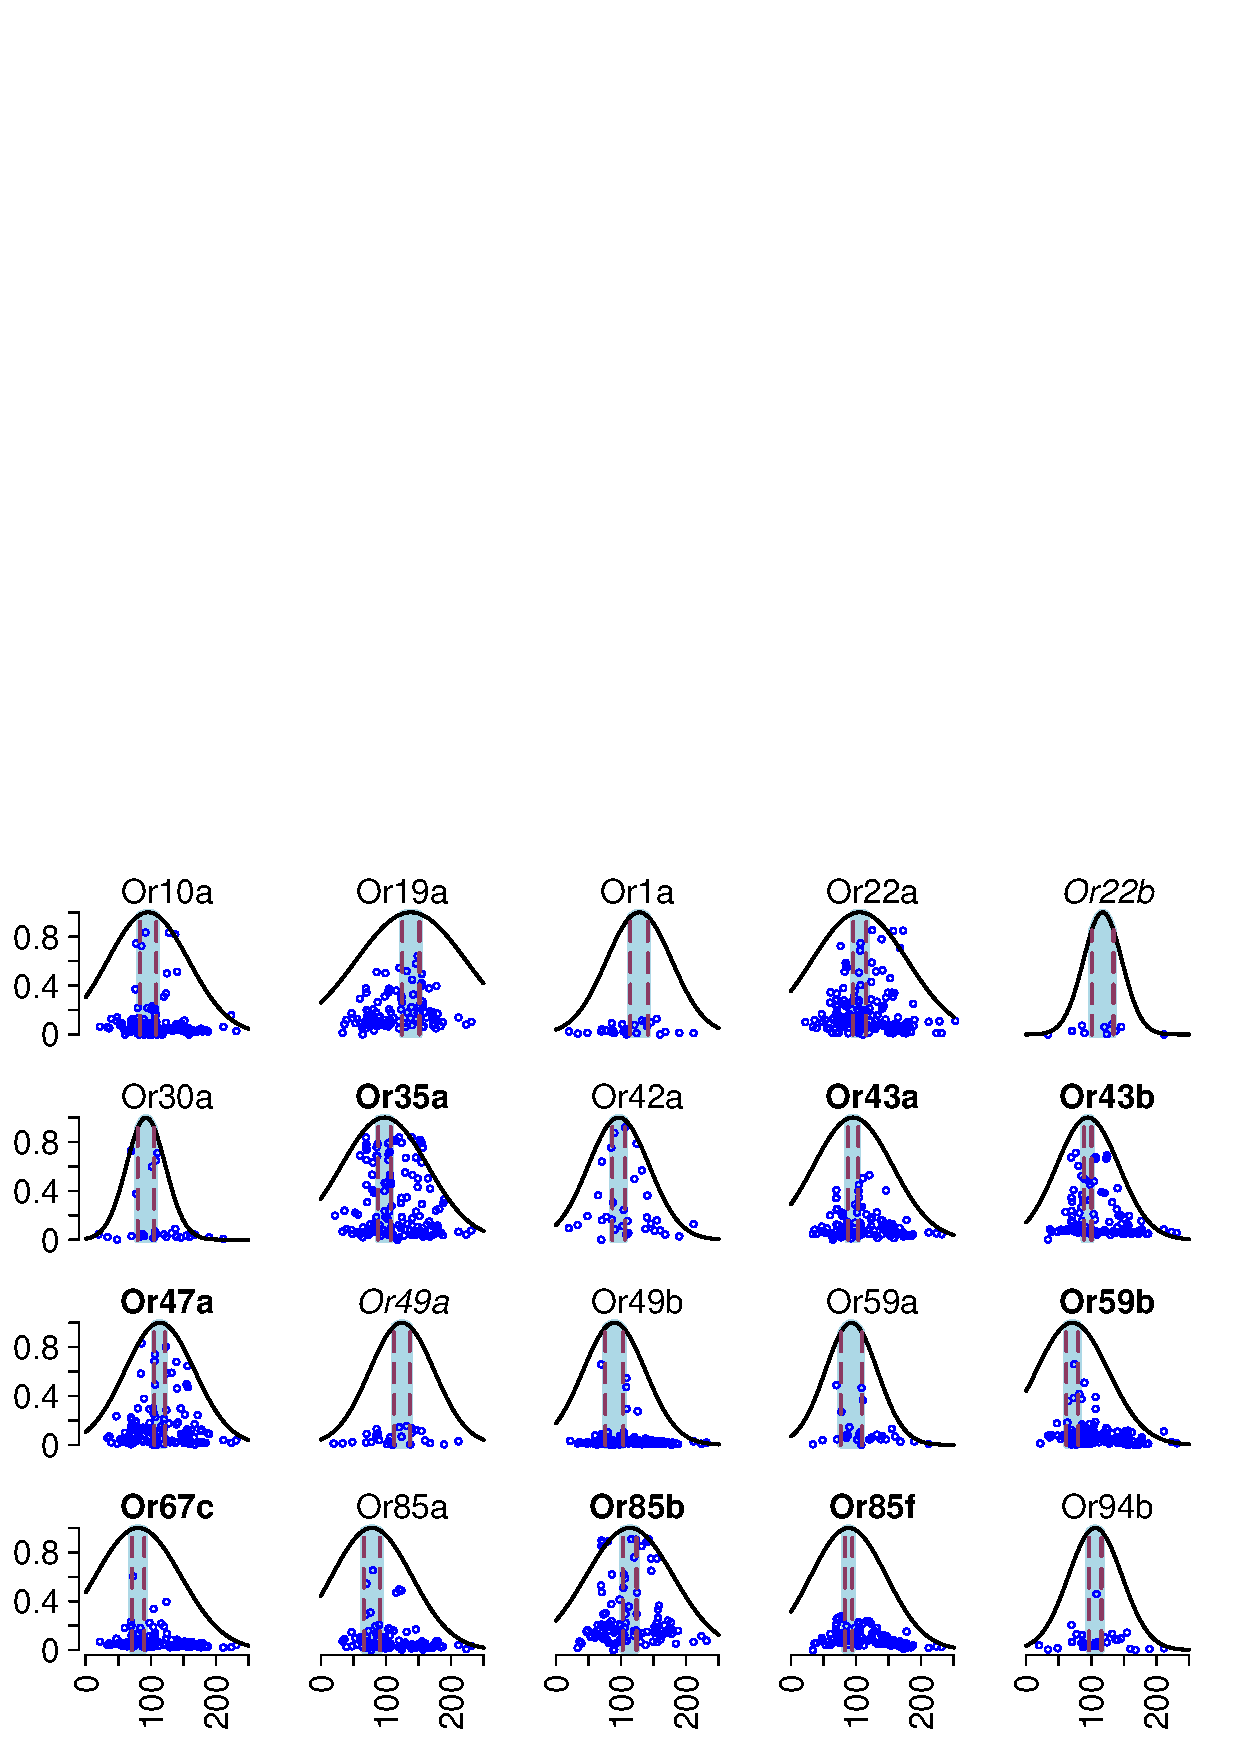
\includegraphics[width=\textwidth]{fig/vol-res}
		\caption{}
		\label{fig:vol-res:all}		
	\end{subfigure}
	\begin{subfigure}[b]{0.75 \textwidth}
		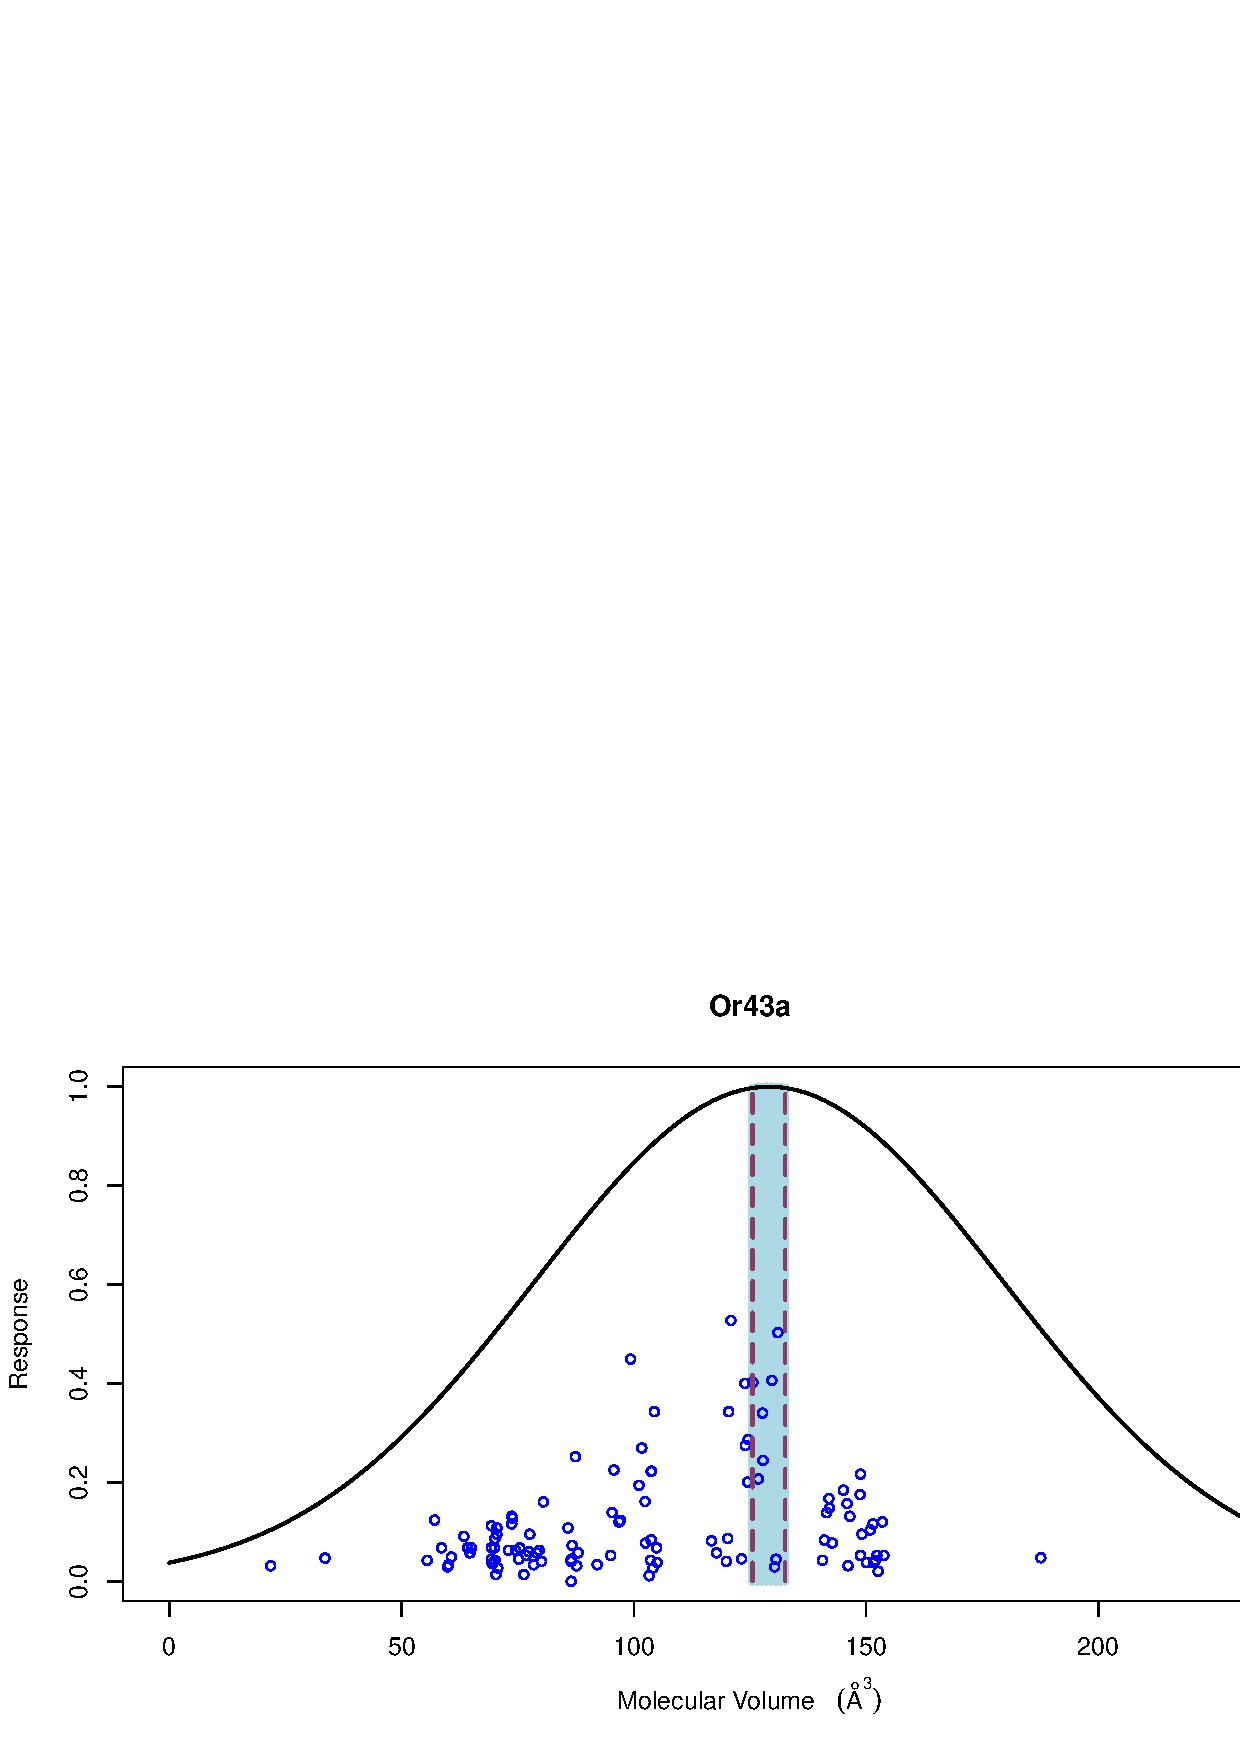
\includegraphics[width= \textwidth]{fig/vol-res-Or43a}
		\caption{}	
		\label{fig:vol-res:one}	
	\end{subfigure}
	\caption{Response of odor-receptors  versus molecular volume of odorants (Circles), the fitted functions $f_n(v)$ from Eq. \ref{eqn:factors} (solid lines), 
		and the error bars of the mean of $f_n(v)$ (red vertical lines),
		for all \numberofreceptors receptors Fig. \ref{fig:vol-res:all} and for one selected receptor Or43a Fig. \ref{fig:vol-res:one} to demonstrate the details. }
	\label{fig:vol-res}
\end{figure}•
\begin{figure}
	\begin{subfigure}[b]{\textwidth}
		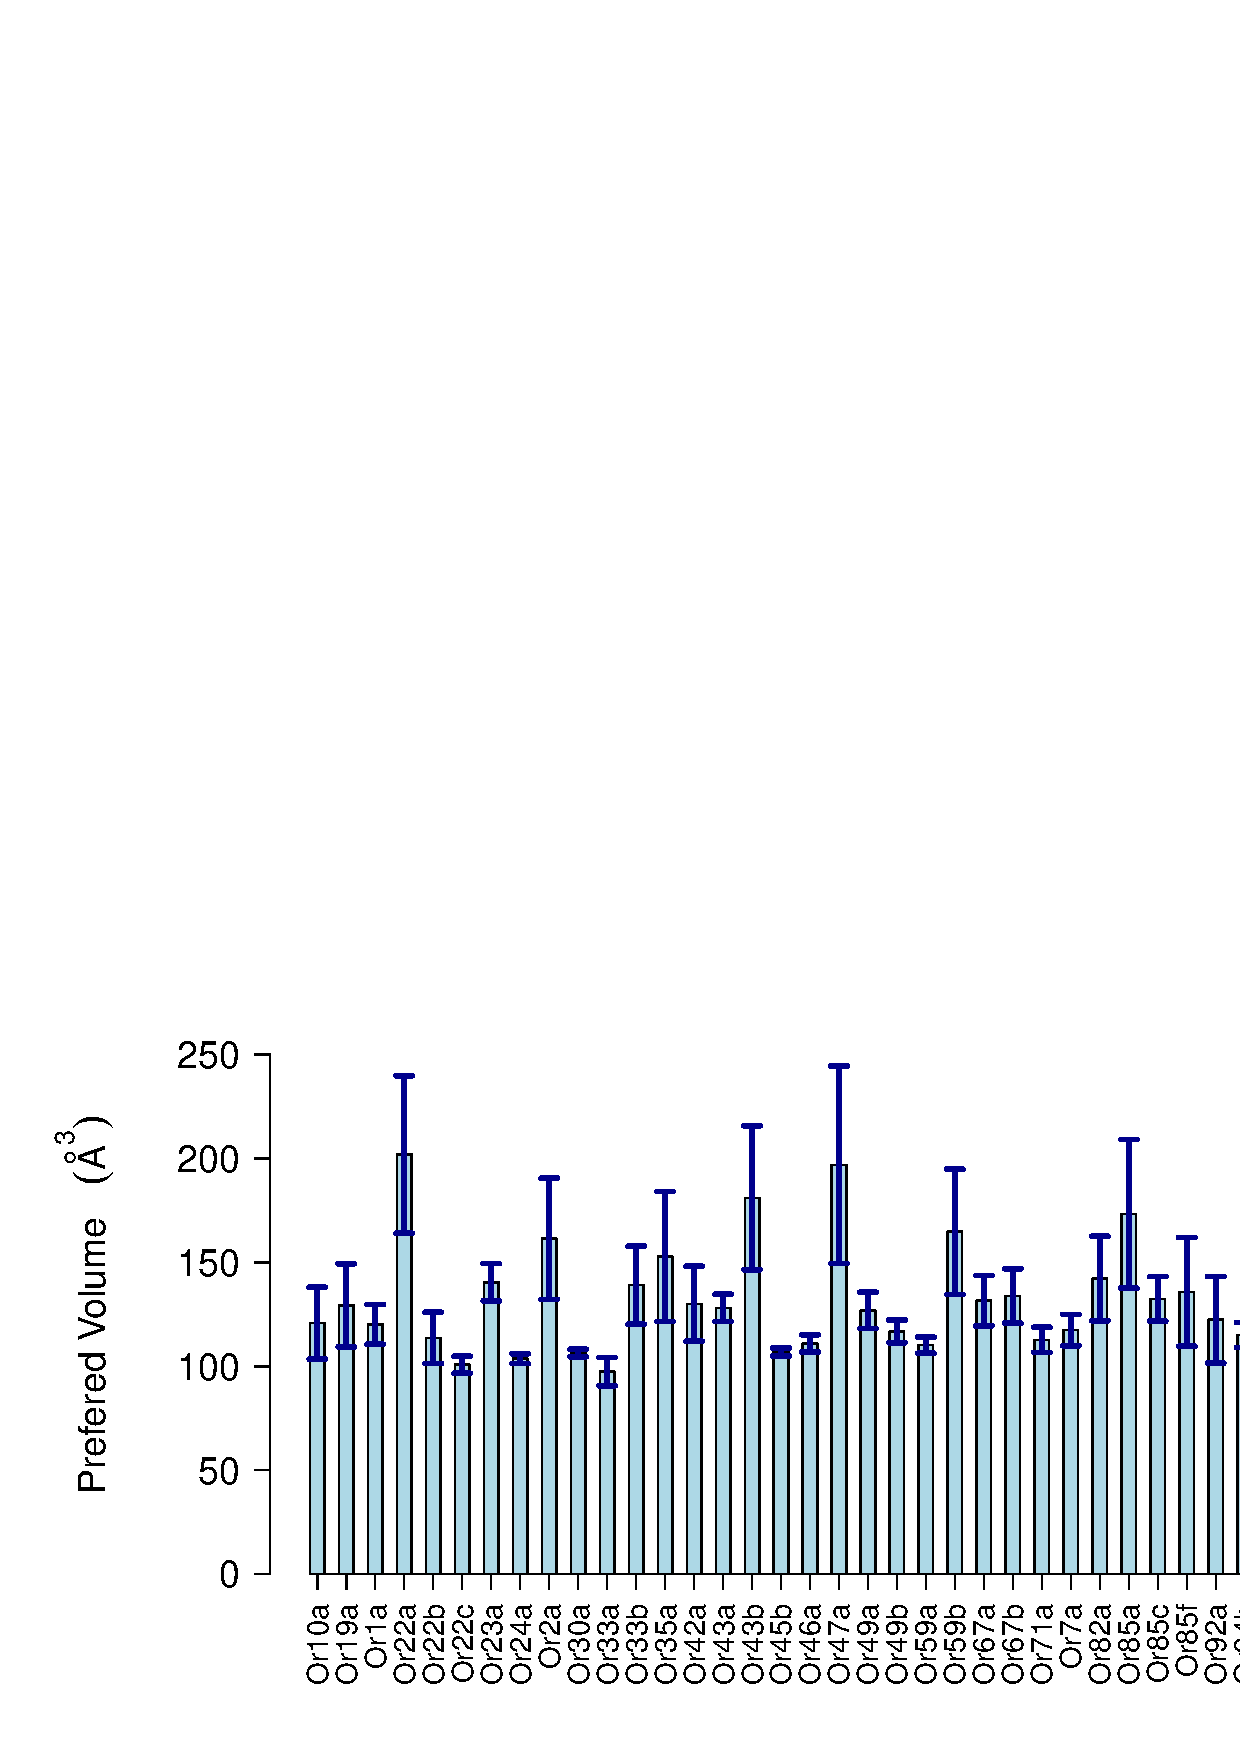
\includegraphics[width=\textwidth]{fig/mean-vol}
		\caption{The prefered volumes of \numberofreceptors receptors ($v_n$), and their error bars. Error bars are calculated using Jack-Knife method. 
		The volume of binding-pocket varies across receptors. 
		Some receptors binds to smaller molecules (Or52b) but some other receptors prefer larger molecules (Or13a and Or98a).}
		\label{fig:preferred_volume}
	\end{subfigure}
	\begin{subfigure}[b]{\textwidth}
		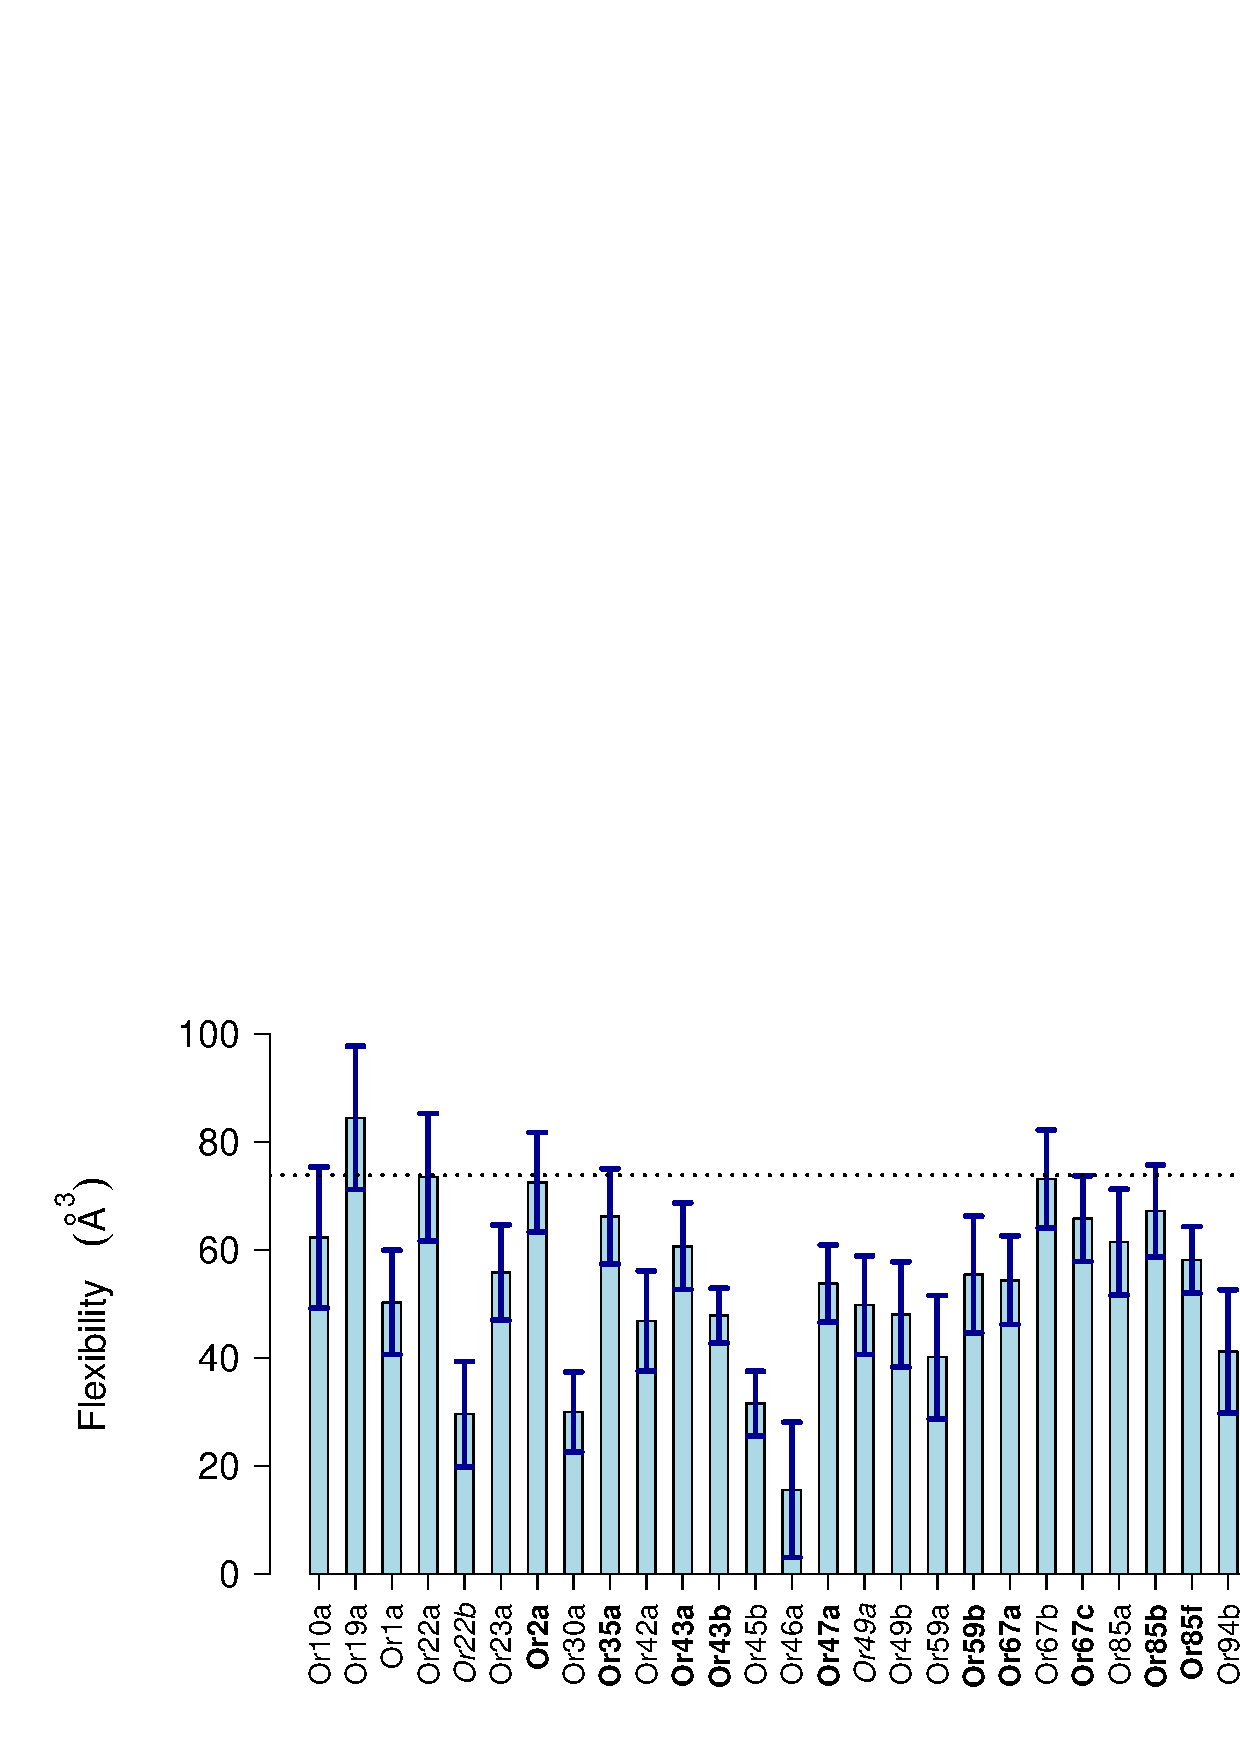
\includegraphics[width=\textwidth]{fig/std-vol}
		\caption{The flexibility of each receptor ($\sigma_n$), the error bars are calculated using Jack-Knife method.
		Some receptors like Or30a are more volume selective but some other receptors like Or13a and Or42b are less sensitive toward the molecular volumes.
		This might be due to mechanical flexibility of the binding-pocket.}
		\label{fig:volume_flexibility}
	\end{subfigure}
	\caption{}
\end{figure}•

There are two main assumption in this work: 
First we assumed that the response of an olfactory receptor can be factorized into two terms, 
according to (\ref{eqn:factors}).
Second, we assumed that the volume dependence factor $f_n(v_m)$ in (\ref{eqn:factors}) 
have a Gaussian form (Eq. \ref{eqn:volume-dependence}).
Considering the physics and chemistry behind the binding-process (Fig. \ref{fig:binding-pocket}), 
and the neural responses (Fig. \ref{fig:vol-res}), 
these assumptions are logical. 

%but, to be sure, we also put them in a test. 
%After calculating function $f_n(v)$ for each olfactory receptor, we can calculate $\psi_{nm}$ of the equation \ref{eqn:factors}.
%If $\psi_{nm}$ is independent of molecular volumes, it means that the assumptions where justified.

The function $f_n(v)$ can be considered as the tuning curve of olfactory receptor $n$ in response to molecular volume (Fig.~\ref{fig:vol-res}). 
Each receptor has a preferred molecular volume $v_n$ and shows some flexibility $\sigma_n$. 
We calculated the parameters of $f_n(v)$ for \numberofreceptors receptors (Fig. \ref{fig:vol-res}). 
The calculated values, $v_n$ and $\sigma_n$ are in Fig. \ref{fig:preferred_volume} and \ref{fig:volume_flexibility} respectively.
Figure \ref{fig:preferred_volume} demonstrate that the molecular volume preference of receptors are different. 
Figure \ref{fig:volume_flexibility} illustrate that the flexibility of receptors are also different.

Here we showed that the responses of olfactory receptor neurons are related to the molecular volume of odorants, 
apart from that, it is not clear which other features of molecules are measured by olfactory receptors. 
It is a topic of ongoing researches , 
there are many works that try to connect the physio-chemical properties of molecules to the evoked neural response or perceived smells~\cite{Gabler2013,Schmuker2007}.
But the non-linear volume dependence (Eq. \ref{eqn:factors} and Eq. \ref{eqn:volume-dependence})  
may mask important relations between molecules and neural responses.

By considering the effect of molecular volume on the response of olfactory receptor neurons, 
one might discover more subtle dependence between other molecular features and neural responses, by studding $\psi_{nm}$, 
which otherwise would be masked by this non-linear relation $f_n(v)$.

We also predict some {\it in-vivo} structural aspects of  the binding-pocket of olfactory receptors:
the preferred volume of each receptor results from the volume of the binding-pocket,
the flexibility of a receptor results from the rigidity or flexibility of the binding-pocket; 
%Therefore, our results provides information about both structural and dynamical properties of olfactory receptors in Drosophila. 
These data add some constrains over the 3d structure of olfactory receptors, 
which may help the prediction and calculation of 3d structure of these proteins. 

The method of this work can be combined with mutagenesis~\cite{} as well. 
Some genes of an olfactory receptor are mutated, 
then its response to a selection of molecules are measured and finally the preferred volume and flexibility are calculated.
In this way we can understand which amino acids of the olfactory receptor contribute to the volume and flexibility of the binding-pocket, 
as well as affecting the function of the receptors.

Our finding can also save time ans expenses of experiments by suggesting important odorants for every receptors.
To study $\psi_{nm}$ of a receptor, it is better to have many data points and those data points are better to be around the preferred volume of the receptor.
But this is not the case in current data, 
for many receptors, most data points are on the tails of $f_n(v)$, which is close to zero,
and for some others receptors like Or22a, Or43b, Or59b and Or98a, 
the preferred volume is out of the range of current data.
In table \ref{tab:receptor-odorant} we suggested the best selection of odorants for each of \numberofreceptors studied receptors.
\begin{table}
\centering
	\begin{tabular}{|l|r|r|r|}
		\hline 
		Receptor & studied & $v_n \pm \sigma_n$ & proposed\\ \hline 
		Or1a & & & \\
		Or2a & & & \\
		Or3b & & & \\	\hline
	\end{tabular}
	\caption{Based on this study we suggest some odorants to be studied experimentally for each receptors. 		
		The numbers of suggested odorants are in last column and the actual list of odorants are in supporting information.
		These odorants are selected according to their molecular volume, if it is in the range of $v_n \pm \sigma_n$.
		The other columns include the number of studied ordorant for each receptor, 
		the number of studied odorants with a molecular volume in range of $v_n \pm \sigma_n$.}
	\label{tab:receptor-odorant}
\end{table}•

Although this work is on the data of Drosophila, 
we expect that the general principle and methodology of this work hold for vertebrates as well. 
But considering the similarities and dissimilarities between insects and vertebrate, 
this should be verified and more work are necessary.

\section{Acknowledgments}
We are especially grateful to B. N. Araabi, S. Aghvami and N. Doostani for the careful reading of the manuscript; and P. Carloni for the fruitful discussion.

\printbibliography
\end{document}
